%% Przykład #1 pracy magisterskiej z pakietem wkmgr
\documentclass[brudnopis,xodstep]{wkmgr}
%%
%% Skład alternatywnymi krojami pisma
%% +--------------------------------+
%% skład fontami podobnymi do kroju Palatino:
% \usepackage{tgpagella,pxfonts,qpxmath} %% pxfonts
%% skład fontami podobnymi do kroju Times:
\usepackage{tgtermes,txfonts,qtxmath} %% txfonts
%%
\usepackage[T1]{fontenc}
\usepackage[utf8]{inputenc}
\usepackage[T1]{polski}
\usepackage{array}

%% podpisy pod rysunkami/tytuły tabel nad tabelami; oba od lewej a nie centrowane ; złożone mniejszym stopniem
\usepackage[font=small,justification=raggedright,singlelinecheck=off,tableposition=top]{caption}

%% klikalne linki w pliku PDF 
%% +------------------------+
%% opcja pagebackref generuje linki w spisie literatury (do strony na której zacytowano pozycję):
\usepackage[breaklinks,pagebackref]{hyperref}
%% \usepackage[breaklinks]{hyperref} %% 

%% Cytowanie autor-rok (pakiet natbib):
%% +---------------------------------+
\usepackage[authoryear]{natbib}
%%
%%
%% Paginy (opcjonalne, odkomentuj poniższe jeżeli mają być dodane):
% \usepackage{fancyhdr}
% \pagestyle{fancyplain}
% \renewcommand{\chaptermark}[1]{\markboth{#1}{}}
% \renewcommand{\sectionmark}[1]{\markright{\thesection{.} #1}}
% \lhead[\fancyplain{}{\renewcommand\familydefault{\rmdefault}%
%       \normalfont \small\itshape\thepage}]
%      {\fancyplain{}{\renewcommand\familydefault{\rmdefault}%
%       \normalfont \small\itshape\rightmark}}
% \rhead[\fancyplain{}{\renewcommand\familydefault{\rmdefault}%
%      \normalfont \small\itshape\leftmark}]
%     {\fancyplain{}{\renewcommand\familydefault{\rmdefault}%
%      \normalfont \small\itshape\thepage}}
% \cfoot[]{}
%%


%%
%% Opcjonalnie identyfikator dokumentu (drukowany tylko z włączoną opcją `brudnopis'):
\nrwersji {0.1}

% Dane autora(ów):
\author{Józef Miśkiewicz}
\nralbumu{0123456789}
\email{walenty@szczesny.com.pl}

%% Jeżeli jest drugi autor:
%% \author{Monika A.~Szczęsna-Woś}
%% \nralbumu{rr000000002}

% Tytuł pracy:
\title{Tytuł pracy}

% Kierunek, tj. katedra/instytut promotora:
\kierunek {Pendologia eksperymentalna}

% Rok obrony:
\date{2011}

% Nazwa szkoły:
\UniversityName{Uniwersytet Kaszubski -- Wydział Pendologii}
% Jeżeli nie podano miejsca zostanie wpisany `Sopot'
\miejsce{Wejherowo}

% Tytuł naukowy, imię i nazwisko promotora:
\opiekun{dr~hab. Jan Kowalski}

%
% Miejsce na deklaracje własnych poleceń:
\newcommand{\filename}[1]{\texttt{#1}}

\def\SITI{SI/TI} %%%
\def\ISTI{SI/TI} %%%
\def\UTAUT{UTAUT} %%%
%%

\makeatletter 
% polecenie zawierające @ muszą być wew \makeatletter ... \makeatother
%% Poprawienie błędu w pakiecie pxfonts.sty
\makeatletter %%
\def\T@n@@nc@d@ngM@cr@M@d{}
\makeatother

\begin{document}

%%
\nocite{beebe,p.perl} %% dołącza niecytowane
%%\nocite{*} %% ** dołącza wszystko **

% Streszczenie/Słowa kluczowe (opcjonalne)
\begin{abstract}
Model Akceptacji Technologii jest najczęściej stosowaną teorią objaśniającą wykorzystanie
i~akceptację systemów informacyjnych w~praktyce badawczej Informatyki Ekonomicznej
\end{abstract}
%% Jeżeli nie ma być słów kluczowych nie wstawiaj deklaracji \keywords{...}
%% uwaga: polecenie \keywords{} z `pustym' argumentem nie zadziała
%%\keywords{SGML, XML, XSL, dokumenty elektroniczne, dokumenty strukturalne}

% Tytuł/spis treści
\maketitle
%

\introduction

Wstęp o~objętości 3--5 stron winien zawierać: 

ogólne wprowadzenie do problemu rozpatrywanego w~pracy:

opis problemu badawczego, określenie celu pracy (pytań/problemów badawczych);

postawienie hipotez;

określenie zakresu pracy, metod, technik i~narzędzi badawczych, 

omówienie konstrukcji pracy.

%%
\chapter{Tytuł rozdziału pierwszego}
\section{Tytuł punktu pierwszego}

Treść punktu jeden, treść punktu jeden, treść punktu jeden, treść punktu jeden.
Treść punktu jeden, treść punktu jeden, treść punktu jeden, treść punktu jeden.
Treść punktu jeden, treść punktu jeden, treść punktu jeden, treść punktu jeden.
Treść punktu jeden, treść punktu jeden, treść punktu jeden, treść punktu jeden.

\subsection{Tytuł podpunktu pierwszego}

Treść punktu dwa, treść punktu dwa, treść punktu dwa, treść punktu dwa.
Treść punktu dwa, treść punktu dwa, treść punktu dwa, treść punktu dwa.
Treść punktu dwa, treść punktu dwa, treść punktu dwa, treść punktu dwa.
Treść punktu dwa, treść punktu dwa, treść punktu dwa, treść punktu dwa.

Treść punktu dwa, treść punktu dwa, treść punktu dwa, treść punktu dwa.
Treść punktu dwa, treść punktu dwa, treść punktu dwa, treść punktu dwa.
Treść punktu dwa, treść punktu dwa, treść punktu dwa, treść punktu dwa.
Treść punktu dwa, treść punktu dwa, treść punktu dwa, treść punktu dwa.

\subsection{Tytuł podpunktu drugiego}

%% więcej podpunktów nie ma -- odkomentuj poniższe a LaTeX zgłosi błąd:
%% \subsubsection{Tytuł podpunktu drugiego}

Treść punktu trzy, treść punktu trzy, treść punktu trzy, treść punktu trzy.
Treść punktu trzy, treść punktu trzy, treść punktu trzy, treść punktu trzy.
Treść punktu trzy, treść punktu trzy, treść punktu trzy, treść punktu trzy.
Treść punktu trzy, treść punktu trzy, treść punktu trzy, treść punktu trzy.

Treść punktu trzy, treść punktu trzy, treść punktu trzy, treść punktu trzy.
Treść punktu trzy, treść punktu trzy, treść punktu trzy, treść punktu trzy.
Treść punktu trzy, treść punktu trzy, treść punktu trzy, treść punktu trzy.
Treść punktu trzy, treść punktu trzy, treść punktu trzy, treść punktu trzy.

Treść punktu trzy, treść punktu trzy, treść punktu trzy, treść punktu trzy.
Treść punktu trzy, treść punktu trzy, treść punktu trzy, treść punktu trzy.
Treść punktu trzy, treść punktu trzy, treść punktu trzy, treść punktu trzy.
Treść punktu trzy, treść punktu trzy, treść punktu trzy, treść punktu trzy.


\section{Tytuł punktu drugiego}

Treść punktu cztery, treść punktu cztery, treść punktu cztery, treść punktu cztery.
Treść punktu cztery, treść punktu cztery, treść punktu cztery, treść punktu cztery.
Treść punktu cztery, treść punktu cztery, treść punktu cztery, treść punktu cztery.
Treść punktu cztery, treść punktu cztery, treść punktu cztery, treść punktu cztery.

Treść punktu cztery, treść punktu cztery, treść punktu cztery, treść punktu cztery.
Treść punktu cztery, treść punktu cztery, treść punktu cztery, treść punktu cztery.
Treść punktu cztery, treść punktu cztery, treść punktu cztery, treść punktu cztery.
Treść punktu cztery, treść punktu cztery, treść punktu cztery, treść punktu cztery.

\section{Tytuł punktu trzeciego}

Treść punktu pięć, treść punktu pięć, treść punktu pięć, treść punktu pięć.
Treść punktu pięć, treść punktu pięć, treść punktu pięć, treść punktu pięć.
Treść punktu pięć, treść punktu pięć, treść punktu pięć, treść punktu pięć.
Treść punktu pięć, treść punktu pięć, treść punktu pięć, treść punktu pięć.

Treść punktu pięć, treść punktu pięć, treść punktu pięć, treść punktu pięć.
Treść punktu pięć, treść punktu pięć, treść punktu pięć, treść punktu pięć.
Treść punktu pięć, treść punktu pięć, treść punktu pięć, treść punktu pięć.
Treść punktu pięć, treść punktu pięć, treść punktu pięć, treść punktu pięć.

Treść punktu pięć, treść punktu pięć, treść punktu pięć, treść punktu pięć.
Treść punktu pięć, treść punktu pięć, treść punktu pięć, treść punktu pięć.
Treść punktu pięć, treść punktu pięć, treść punktu pięć, treść punktu pięć.
Treść punktu pięć, treść punktu pięć, treść punktu pięć, treść punktu pięć.

Treść punktu pięć, treść punktu pięć, treść punktu pięć, treść punktu pięć.
Treść punktu pięć, treść punktu pięć, treść punktu pięć, treść punktu pięć.
Treść punktu pięć, treść punktu pięć, treść punktu pięć, treść punktu pięć.
Treść punktu pięć, treść punktu pięć, treść punktu pięć, treść punktu pięć.


\section{Tytuł podpunktu pierwszego}

Treść punktu sześć, treść punktu sześć, treść punktu sześć, treść punktu sześć.
Treść punktu sześć, treść punktu sześć, treść punktu sześć, treść punktu sześć.
Treść punktu sześć, treść punktu sześć, treść punktu sześć, treść punktu sześć.
Treść punktu sześć, treść punktu sześć, treść punktu sześć, treść punktu sześć.

Treść punktu sześć, treść punktu sześć, treść punktu sześć, treść punktu sześć.
Treść punktu sześć, treść punktu sześć, treść punktu sześć, treść punktu sześć.
Treść punktu sześć, treść punktu sześć, treść punktu sześć, treść punktu sześć.
Treść punktu sześć, treść punktu sześć, treść punktu sześć, treść punktu sześć.

Treść punktu sześć, treść punktu sześć, treść punktu sześć, treść punktu sześć.
Treść punktu sześć, treść punktu sześć, treść punktu sześć, treść punktu sześć.
Treść punktu sześć, treść punktu sześć, treść punktu sześć, treść punktu sześć.
Treść punktu sześć, treść punktu sześć, treść punktu sześć, treść punktu sześć.

Treść punktu sześć, treść punktu sześć, treść punktu sześć, treść punktu sześć.
Treść punktu sześć, treść punktu sześć, treść punktu sześć, treść punktu sześć.
Treść punktu sześć, treść punktu sześć, treść punktu sześć, treść punktu sześć.
Treść punktu sześć, treść punktu sześć, treść punktu sześć, treść punktu sześć.


\section{Tytuł podpunktu drugiego}

Treść punktu siedem, treść punktu siedem, treść punktu siedem, treść punktu siedem.
Treść punktu siedem, treść punktu siedem, treść punktu siedem, treść punktu siedem.
Treść punktu siedem, treść punktu siedem, treść punktu siedem, treść punktu siedem.
Treść punktu siedem, treść punktu siedem, treść punktu siedem, treść punktu siedem.

Treść punktu siedem, treść punktu siedem, treść punktu siedem, treść punktu siedem.
Treść punktu siedem, treść punktu siedem, treść punktu siedem, treść punktu siedem.
Treść punktu siedem, treść punktu siedem, treść punktu siedem, treść punktu siedem.
Treść punktu siedem, treść punktu siedem, treść punktu siedem, treść punktu siedem.

Treść punktu siedem, treść punktu siedem, treść punktu siedem, treść punktu siedem.
Treść punktu siedem, treść punktu siedem, treść punktu siedem, treść punktu siedem.
Treść punktu siedem, treść punktu siedem, treść punktu siedem, treść punktu siedem.
Treść punktu siedem, treść punktu siedem, treść punktu siedem, treść punktu siedem.

Treść punktu siedem, treść punktu siedem, treść punktu siedem, treść punktu siedem.
Treść punktu siedem, treść punktu siedem, treść punktu siedem, treść punktu siedem.
Treść punktu siedem, treść punktu siedem, treść punktu siedem, treść punktu siedem.
Treść punktu siedem, treść punktu siedem, treść punktu siedem, treść punktu siedem.

Treść punktu siedem, treść punktu siedem, treść punktu siedem, treść punktu siedem.
Treść punktu siedem, treść punktu siedem, treść punktu siedem, treść punktu siedem.
Treść punktu siedem, treść punktu siedem, treść punktu siedem, treść punktu siedem.
Treść punktu siedem, treść punktu siedem, treść punktu siedem, treść punktu siedem.

Treść punktu siedem, treść punktu siedem, treść punktu siedem, treść punktu siedem.
Treść punktu siedem, treść punktu siedem, treść punktu siedem, treść punktu siedem.
Treść punktu siedem, treść punktu siedem, treść punktu siedem, treść punktu siedem.
Treść punktu siedem, treść punktu siedem, treść punktu siedem, treść punktu siedem.


%%
\chapter{Model Akceptacji Technologii \label{TAM-def-punkt}}
\section{Podstawowe informacje \label{TAM-def}}

Model Akceptacji Technologii (\emph{Technology Acceptance Model}, TAM)
jest najczęściej stosowaną teorią objaśniającą wykorzystanie
i~akceptację systemów informacyjnych w~praktyce badawczej Informatyki
Ekonomicznej~\citep{VenkateshEtAl03,VenkateshDavis00}.
Lee i inni~\citeyearpar{LeeKozarLarsen2003} określają model TAM jak
,,najczęściej stosowaną teorię opisującą 
indywidualną akceptację systemów informacyjnych''.
Model TAM został zaadaptowany z~rozwiniętej na gruncie psychologii
społecznej teorii uzasadnionego działania 
Ajzena i~Fishbeina (\emph{Theory of Reasoned Action},
TRA) i~teorii planowanego 
działania (\emph{Theory of Planned Behaviour}, TPB) 
będącej jej
rozwinięciem~\citep{FishbeinAjzen1975,Ajzen1991}.
Według teorii uzasadnionego działania
działanie poprzedza \emph{intencja}, która z~kolei
kształtuje się pod wpływem dwóch czynników: \emph{subiektywnej
  normy\/}\footnote{Subiektywne normy
  (SN, \emph{subjective norms\/}) to ,,przekonania jednostki na ile jej
  działania będą akceptowane na tak lub nie przez ważne dla tej
  jednostki osoby''~(\citet[s.~302]{Ajzen1991} za Venkateshem i~Davisem~\citeyearpar[s.~187]{VenkateshDavis00}).}
oraz~\emph{postawy\/}\footnote{Postawa względem zachowania
  (ATT, \emph{attitude toward behaviour\/}), to przekonania względem
  konsekwencji zachowania oraz ocena tych konsekwencji dla jednostki.}
względem tego zachowania.  Wreszcie postawy wynikają z~przekonań
(\emph{beliefs\/}) względem użytkowania (systemów informacyjnych w~tym
przypadku). 
Teoria planowanego działania
jest rozszerzeniem TRA i~zakłada, że działania kształtuje
oprócz norm subiektywnych i~postaw także trzeci 
czynnik określany jako \emph{postrzegana kontrola 
behawioralna\/}\footnote{Postrzegana kontrola 
behawioralna\label{TPB-def} (PBC), to
przekonanie co do możliwości wykonania działania~\citep{Ajzen-tpb-www}.
Ajzen \citeyearpar[s.~18]{Ajzen1991}
wskazuje na podobieństwo PBC z~czynnikiem samoskuteczności
z~teorii społecznego uczenia~\citep{Bandura1994}. }.
PBC jest wykorzystywany w~rozszerzonych wersjach modelu TAM, 
por.~przykładowo~\cite{VenkateshEtAl03} lub~\cite{MathiesonEtAl01}.

TRA/TBP to ogólny model zachowania a~jego konkretyzacja
polega m.in. na określeniu przekonań, które są istotne dla zachowania
będącego przedmiotem zainteresowania badacza. Inne przekonania
determinują palanie bądź nie palenie tytoniu a~inne używanie bądź nie
używanie aplikacji komputerowych.  Davis postuluje, że kluczową rolę
odgrywają dwa przekonania\footnote{Ajzen i~Fishbein rekomendują więcej
  -- od pięciu do dziewięciu
  przekonań~\citep[s.~218]{FishbeinAjzen1975}.} nazwane przez niego
postrzegana użyteczność \emph{preceived
  usefulness\/}) oraz postrzegana łatwość
użytkowania (PEOU, \emph{perceived ease of~use\/}).

Pierwsze przekonanie jest określone
jako ,,stopień przekonania użytkownika, że korzystanie z~określonego
systemu zwiększy jego efektywność
pracy''~\citep{DavisetAl1989,Davis1989}.  Z~kolei postrzegana łatwość
użytkowania jest definiowana jako ,,stopień przekonania użytkownika,
że korzystanie z~określonego systemu będzie
łatwe''~\citep{DavisetAl1989,Davis1989}. Skale pomiarowe dla obu
czynników zostały opracowane i~zweryfikowane w~pracach
Davisa i~innych~\citeyearpar{Davis1989} oraz Adamsa i~innych~\citeyearpar{AdamsNelsonTodd1992}.
Reasumując:
,,klasyczny'' model TAM zawiera pięć czynników
(por.~rys.~\ref{r1-TAM}): postrzegana użyteczność (PU), postrzegana
łatwość użytkowania (PEOU), postawa wobec używania (ATT), intencja
używania (BI) oraz wykorzystanie (USE)\footnote{Czynniki ATT oraz BI
  są wprost zaadaptowane z~modeli TRA/TPB.}.

\begin{figure}[!tbh]
  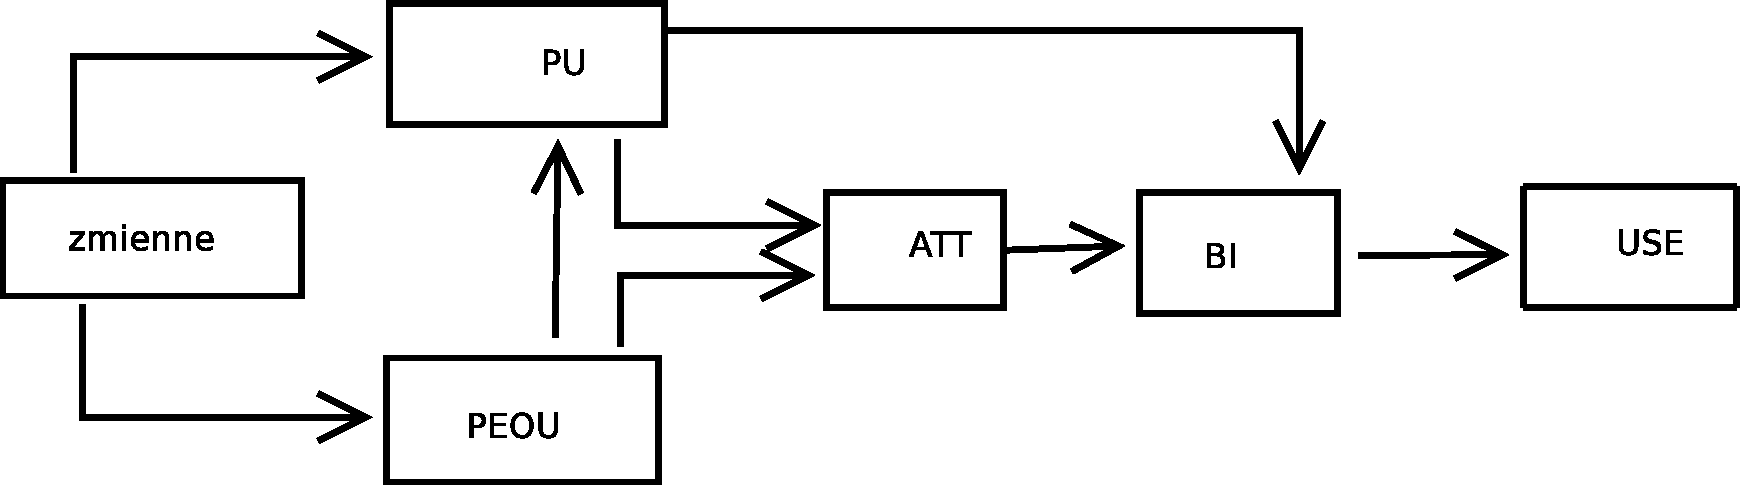
\includegraphics[width=\textwidth]{./TAM-pl}
%%\caption[Model Akceptacji Technologii]{Model Akceptacji Technologii, opracowanie własne za~\cite{DavisetAl1989}}
\caption{Model Akceptacji Technologii}
\source{opracowanie własne za:~\cite{DavisetAl1989}}
\label{r1-TAM}
\end{figure}

Model TAM nie zawiera czynnika
\emph{norm subiektywnych}, który to czynnik jest według hipotez
TRA/TBP istotnym determinantem intencji~(\citet{FishbeinAjzen1975},
\citet[s.~150]{TaylorTodd95} oraz \citet[s.~59--60]{Burton-JonesHubona05}).
Davis \citeyearpar[s.~986]{DavisetAl1989} uprościł swój model usuwając z~niego czynnik \emph{norm
  subiektywnych\/} ponieważ, po pierwsze ich wpływ
w~przeprowadzonych przez niego eksperymentach nie był znaczący, 
a~po drugie
stosowane do pomiaru \emph{norm subiektywnych\/} skale psychometryczne
były w~jego opinii słabe\footnote{Ta decyzja była
  słuszna w~sytuacji nasycenie organizacji w~technologię IT było
  niskie, gdy użytkownicy posługiwali się prostymi systemami, a~ich
  wykorzystanie w~organizacji było dobrowolne -- typowa sytuacji
  w~końcu lat osiemdziesiątych. 
Powstaje pytanie na ile sytuacja powyższa jest w~dalszym ciągu aktualna--współcześnie
typowe jest raczej posługiwanie się aplikacjami wymagającymi uprzedniego
intensywnego szkolenia a~do korzystania z~której pracownik jest zobowiązany. 
Przykładami niech będą systemy zarządzania organizacją typu ERP czy systemy 
EDI/IOS pozwalające
na wymianę danych pomiędzy organizacjami.}. 
Teoria TRA/TBP zakłada ponadto, że przekonania wyjaśniają 
intencje \emph{wyłącznie\/}, za pośrednictwem norm subiektywnych i~postawy 
(oraz kontroli behawioralnej w~przypadku TPB)\footnote{Innymi słowy 
 normy subiektywne i~postawy w~całości mediują wpływ zmiennych zewnętrznych.} podczas gdy w~oryginalnym
modelu TAM (por.~rys.~\ref{r1-TAM}) 
postulowana jest  statystycznie istotna bezpośrednia zależność także pomiędzy PU-BI.
Późniejsze badania potwierdziły empirycznie, że istotnie w~modelu TAM istnieje związek pomiędzy
PU-BI. W rezultacie w~późniejszych wersjach modelu TAM postawy (ATT)
zostały usunięte a czynniki
PU/PEU determinują bezpośrednio intencje\footnote{Por. 
przykładowo \cite{IgbariaetAl97,Burton-JonesHubona05,VenkateshDavis00}.}.

\begin{table}[!tbh]\small
\caption{Opisowe statystyki dla podstawowych relacji z~modelu TAM}
\label{tab:ES-TAM}
\begin{tabular*}{\textwidth}{@{\extracolsep{\stretch{1}}}lrrrr} \hline
Czynniki   & l.~badań  & $r_{\rm min}$ & $r_{\rm max}$ & $\bar r$ \\ \hline
PU-USE     &  72 & -0,41 &  0,91  & 0,40 \\
PEOU-USE   &  61 & -0,20 &  0,98  & 0,29 \\ 
PEOU-PU    & 123 & -0,26 &  0,81  & 0,44 \\ \hline
\end{tabular*}
\source{\cite{ShumailaetAl2007b}}
\end{table}

TAM zakłada, że \emph{zmienne zewnętrzne\/} (charakterystyka systemu IT,
charakterystyka użytkownika, czynniki organizacyjne) wpływają
\emph{pośrednio\/} na intencje determinując wielkość 
%% Uwaga: poniższy odsyłacz jest przeniesiony pomiędzy stronami (por. plik wkmgr1.pdf)
%% co powoduje, że dynamiczny link (generowany przez pakiet hyperref)
%% nie kończy się na brzegu ostatniego wiersza strony poprzedniej,
%% ale obejmuje także ewentualne przypisy, ew. paginę dolną oraz paginę 
%% górną na stronie następnej. Usunięcie breaklinks z listy opcji pakietu 
%% hyperref usunęłoby problem,
%% ale wprowadziłoby inny jednocześnie (nadmierne odstępy w wierszu):
PU/PEOU~\cite[s.~187]{VenkateshDavis00},
przy czym wpływ czynnika PU jest większy niż PEOU. Ponadto wykorzystanie {\SITI}
może być przewidywane na podstawie intencji.
Zamiarem Davisa było opracowanie  ,,prostego, teoretycznie 
uzasadnionego modelu, zdolnego do objaśnienia czynników 
akceptacji systemów komputerowych w~sposób ogólny, to jest dla różnych grup użytkowników
końcowych i~różnych rodzajów systemów [...] TAM ma stanowić teoretyczną
podstawę objaśniającą w~jaki sposób zewnętrzne czynniki wpływają 
na przekonania, postawy i~intencje''~\cite[s.~985]{Davis1989}.
Z~uwagi na trudność z~pomiarem użytkowania systemu wiele badań posługuje się
modelem czteroskładnikowym zakładającym, 
że wysoka 
wartość BI determinuje wysoką wartość użytkowania.

%% %% %% 
\chapter{Tytuł rozdziału trzeciego}

\section{Tytuł punktu pierwszego}

Współcześnie organizacje rzadko posiadają wiedzę i~zasoby niezbędne do
realizacji pierwszych dwóch faz.  Oprogramowanie jest wytwarzane przez
zewnętrznych --~z~punktu widzenia organizacji --~\emph{dostawców},
a~\emph{uruchamiane} przez
\emph{konsultantów\/} oraz \emph{integratorów}\footnote{%%
 Integrator kupuje, instaluje i~testuje aplikacje 
 oraz sprzęt, podczas gdy rolą konsultantów jest 
 wyłącznie doradztwo~\citep{MesserschmittSzyperski03}.}.  
Faza
\emph{uruchamiania\/} obejmuje nie tylko zakup sprzętu
i~oprogramowania, ale także 
usługi doradcze 
i~\emph{integrację}, co oznacza instalację,
testowanie, dostosowanie wewnętrznych procesów organizacji
oraz niezbędne szkolenia. 
Wynikiem 
jest system gotowy do działania.
Eksploatacja z~kolei, to zapewnienie bezawaryjnej pracy systemu,
w~tym pomoc użytkownikom końcowym. 
Zwykle organizacja zatrudnia w~tym celu wyszkolonych 
pracowników 
lub najmuje firmę zewnętrzną.  
Program z~reguły jest wykorzystywany na podstawie \emph{umowy licencyjnej\/}
(por.~punkt~\ref{sec:cpr-lic}), stąd przychody z~fazy
implementacji można utożsamiać z~przychodami z~tytułu udzielonych
licencji.  Tabela~\ref{tab:valimaki} pokazuje 
udział przychodów z~tytułu opłat licencyjnych
 i~usług w~wybranych 
przedsiębiorstwach sektora {\SITI}.

\begin{table}[!tbh]\small
\caption{Przychody z~tytułu licencji i~usług 
 na przykładzie wybranych przedsiębiorstw sektora {\SITI}  w~2004~r.}
\label{tab:valimaki}
\begin{tabular*}{\textwidth}{@{\extracolsep{\stretch{1}}}lrrl} \hline
Nazwa firmy & Licencje$^{\rm a}$ & Przychody$^{\rm b}$ & Produkowane oprogramowanie \\ \hline
Adobe\index{Adobe Inc.} & 98 &  1,7 & DTP, grafika \\
Symantec & 98 &  1,8 &  zabezpieczenie systemów {\SITI}\\ 
Microsoft\index{Microsoft} & 94 & 31,5 & system operacyjny, aplikacje \\ %%\hline
Oracle & 79 & 10,1 & bazy danych, aplikacje korporacyjne \\
CA & 69 &  3,2 & aplikacje korporacyjne \\ 
Siebel & 36 &  1,3 & aplikacje korporacyjne \\
SAP & 31 &  9,7 & aplikacje korporacyjne \\
Novell & 26 &  1,1 & system operacyjny, aplikacje \\
IBM & 25 & 61,3 & sprzęt, aplikacje korporacyjne \\ \hline
\end{tabular*}
\begin{footnotesize}
$^{\rm a}$udział przychodów z~tytułu opłat 
licencyjnych w~\%; $^{\rm b}$roczny przychód w~mld USD 
\end{footnotesize}
\source{opracowanie własne na podstawie:~\citet[s.~28]{Valimaki2005}}
\end{table}

Dane zawarte w~tabeli~\ref{tab:valimaki} pokazują, że przychód
niektórych przedsiębiorstw praktycznie w~całości pochodzi z~opłat
licencyjnych.  Przykładowo 94\% przychodu firmy
Microsoft\index{Microsoft} pochodzi z~licencji; co więcej --~80\%
przychodów i~100\% zysku pochodzi ze sprzedaży zaledwie trzech
programów: systemu Windows na rynku masowym i~korporacyjnym oraz
oprogramowania biurowego MS~Office~\cite[s.~55]{Cusumano2004}.
Z~kolei działająca na rynku korporacyjnym firma SAP osiąga aż 70\% przychodów
z~tytułu usług związanych ze sprzedawanym oprogramowaniem.
Te różnice implikują strategię rynkową firmy, w~tym wykorzystanie
oprogramowania \emph{Open Source}, które --~co pokażemy dalej
--~w~dużym stopniu wyklucza strategie rynkowe
oparte na przychodach z~tytułu 
opłat licencyjnych~\citep[s.~28]{Valimaki2005}.

\section{Tytuł punktu drugiego \label{sec:cpr-lic}}

Treść punktu dwa, treść punktu dwa, treść punktu dwa, treść punktu dwa.
Treść punktu dwa, treść punktu dwa, treść punktu dwa, treść punktu dwa.
Treść punktu dwa, treść punktu dwa, treść punktu dwa, treść punktu dwa.
Treść punktu dwa, treść punktu dwa, treść punktu dwa, treść punktu dwa.

Treść punktu dwa, treść punktu dwa, treść punktu dwa, treść punktu dwa.
Treść punktu dwa, treść punktu dwa, treść punktu dwa, treść punktu dwa.
Treść punktu dwa, treść punktu dwa, treść punktu dwa, treść punktu dwa.
Treść punktu dwa, treść punktu dwa, treść punktu dwa, treść punktu dwa.

\chapter{Tytuł rozdziału czwartego}

\section{Tytuł punktu pierwszego}

Treść punktu jeden, treść punktu jeden, treść punktu jeden, treść punktu jeden.
Treść punktu jeden, treść punktu jeden, treść punktu jeden, treść punktu jeden.
Treść punktu jeden, treść punktu jeden, treść punktu jeden, treść punktu jeden.
Treść punktu jeden, treść punktu jeden, treść punktu jeden, treść punktu jeden.

Treść punktu jeden, treść punktu jeden, treść punktu jeden, treść punktu jeden.
Treść punktu jeden, treść punktu jeden, treść punktu jeden, treść punktu jeden.
Treść punktu jeden, treść punktu jeden, treść punktu jeden, treść punktu jeden.
Treść punktu jeden, treść punktu jeden, treść punktu jeden, treść punktu jeden.

\section{Tytuł punktu drugiego}

Treść punktu dwa, treść punktu dwa, treść punktu dwa, treść punktu dwa.
Treść punktu dwa, treść punktu dwa, treść punktu dwa, treść punktu dwa.
Treść punktu dwa, treść punktu dwa, treść punktu dwa, treść punktu dwa.
Treść punktu dwa, treść punktu dwa, treść punktu dwa, treść punktu dwa.

Treść punktu dwa, treść punktu dwa, treść punktu dwa, treść punktu dwa.
Treść punktu dwa, treść punktu dwa, treść punktu dwa, treść punktu dwa.
Treść punktu dwa, treść punktu dwa, treść punktu dwa, treść punktu dwa.
Treść punktu dwa, treść punktu dwa, treść punktu dwa, treść punktu dwa.

\summary

Zakończenie zakończenia powinno obejmować:

Zwięzły opis uzyskanych wyników;

Wskazanie na napotkanie trudności i~potencjalne słabości;

Wskazanie na  potencjalnie ciekawe tematy do dalszych badań, które są konsekwencją
wyników uzyskanych przez autora. 

%
% Załączniki (opcjonalnie):
\appendix
\chapter{Tytuł załącznika jeden}

Treść załącznika jeden. Treść załącznika jeden. Treść załącznika jeden
Treść załącznika jeden. Treść załącznika jeden.  Treść załącznika
jeden.

\chapter{Tytuł załącznika dwa}

Treść załącznika dwa. Treść załącznika dwa. Treść załącznika dwa Treść
załącznika dwa. Treść załącznika dwa.  Treść załącznika dwa.


%% %% %% %% %% %% %% %% %% %% %% %% %% %% %% %% %% %% %% %% %% %% %%
\clearpage 
\phantomsection %% << poprawienie linka generowanego przez hyperref
\addcontentsline{toc}{chapter}{\refname}
\begin{thebibliography}{}
  
\bibitem[Adams i~inni(1992)]{AdamsNelsonTodd1992} Adams, D.~A.,
  Nelson, R.~R., i Todd, P.~A. (1992).  Perceived usefulness, ease of
  use, and usage of information technology: a replication.  \emph{MIS
    Quarterly}, 16(2):227--247.
  
\bibitem[Ajzen(1991)]{Ajzen1991} Ajzen, I. (1991).  The theory of
  planned behavior.  \emph{Organizational Behavior and Human Decision
    Processes}, 50(2):179--211.
  
\bibitem[Ajzen, bdw]{Ajzen-tpb-www} Ajzen, I. (bdw).  Theory of
  planned behavior.  \url{http://www.people.umass.edu/aizen/tpb.html}.
  
\bibitem[Bandura(1994)]{Bandura1994} Bandura, A. (1994).
  \emph{Self-efficacy}, volume~4, pages 71--81.  Academic Press, New
  York.  \url{http://www.des.emory.edu/mfp/BanEncy.html}.

\bibitem[Beebe(1995)]{beebe}
Beebe, N. H.~F. (1995).
 Bibliography prettyprinting and syntax checking.
 \emph{TUGBoat}, 14:395--419.
 \url{http://www.gust.org.pl/PDF/BIUL/10/l2html.pdf}.

\bibitem[Burton-Jones i Hubona(2005)]{Burton-JonesHubona05}
Burton-Jones, A. i Hubona, G.~S. (2005).
 Individual differences and usage behaviour: Revisiting a~technology
  acceptance model assumption.
 \emph{Data Base}, 36(2):58--77.

\bibitem[Cusumano(2004)]{Cusumano2004}
Cusumano, M.~A. (2004).
\emph{The Business of Software: What Every Manager, Programmer, and
Entrepreneur Must Know to Thrive and Survive in Good Times and Bad}.
Free Press.

\bibitem[Davis(1989)]{Davis1989}
Davis, F.~D. (1989).
 Perceived usefulness, perceived easy of use, and user acceptance of
  information technology.
 \emph{MIS Quarterly}, 13(3):319--340.

\bibitem[Davis i~inni(1989)]{DavisetAl1989}
Davis, F.~D., Bagozzi, R.~P., i Warshaw, P.~R. (1989).
 User acceptance of computer technology: a comparison of two
  theoretical models.
 \emph{Decision Science}, 35(8):982--1003.

\bibitem[Fishbein i Ajzen(1975)]{FishbeinAjzen1975}
Fishbein, M. i Ajzen, I. (1975).
 \emph{Belief, Attitude, Intention, and Behaviour: An Introduction to
  Theory and Research}.
 Addison-Wesley.

\bibitem[Igbaria i~inni(1997)]{IgbariaetAl97}
Igbaria, M., Zinatelli, N., Cragg, P., i Cavaye, A. L.~M. (1997).
 Personal computing acceptance factors in small firms: A structural
  equation model.
 \emph{MIS Quarterly}, 21(3):279--305.

\bibitem[Lee i~inni(2003)]{LeeKozarLarsen2003}
Lee, Y., Kozar, K.~A., i Larsen, K. R.~T. (2003).
 The technology acceptance model: Past, present and future.
 \emph{Communications of AIS}, 12:752--780.

\bibitem[Mathieson i~inni(2001)]{MathiesonEtAl01}
Mathieson, K., Peacock, E., i Chin, W.~W. (2001).
 Extending the technology acceptance model: The influence of perceived
  user resources.
 \emph{SIGMIS Database}, 32(3):86--112.

\bibitem[Messerschmitt i Szyperski(2003)]{MesserschmittSzyperski03}
Messerschmitt, D.~G. i Szyperski, C. (2003).
\emph{Software Ecosystems: Understanding an Indispensable Technology
and Industry}. {MIT} Press.

\bibitem[Taylor i Todd(1995)]{TaylorTodd95}
Taylor, S. i Todd, P.~A. (1995).
 Understanding information technology usage: A~test of competing
  models.
 \emph{Information Systems Research}, 6(2):144--176.

\bibitem[V{\"a}lim{\"a}ki(2005)]{Valimaki2005}
V{\"a}lim{\"a}ki, M. (2005).
\emph{The Rise of Open Source Licensing. A Challenge to the Use of
  Intellectual Property in the Software Industry}.
Turre Publishing, Helsinki.
\url{pub.turre.com}.

\bibitem[Venkatesh i Davis(2000)]{VenkateshDavis00}
Venkatesh, V. i Davis, F.~D. (2000).
 A theoretical extension of the technology acceptance model: Four
  longitudinal field studies.
 \emph{Management Science}, 46(2):186--204.

\bibitem[Venkatesh i~inni(2003)]{VenkateshEtAl03}
Venkatesh, V., Morris, M.~G., Davis, G.~B., , i Davis, F.~D. (2003).
 User acceptance of information technology: Toward a unified view.
 \emph{MIS Quarterly}, 27(3):425--478.

\bibitem[Wall i~inni(1996)]{p.perl}
Wall, L., Christiansen, T., i Schwartz, R. (1996).
 \emph{Programming Perl}.
 O'Reilly \&~Associates.

\bibitem[Yousafzai i~inni(2007b)]{ShumailaetAl2007b}
Yousafzai, S.~Y., Foxall, G.~R., i Pallister, J.~G. (2007b).
Technology acceptance: a meta-analysis of the {TAM}: Part~2.
{\em Journal of Modelling in Management}, 2.

\end{thebibliography}

%
% Spis tabel (jeżeli jest potrzebny):
\clearpage 
\phantomsection %% << poprawienie linka generowanego przez hyperref
\addcontentsline{toc}{chapter}{\listtablename}
\listoftables


% Spis rysunków (jeżeli jest potrzebny):
\clearpage 
\phantomsection %% << poprawienie linka generowanego przez hyperref
\addcontentsline{toc}{chapter}{\listfigurename}
\listoffigures

\end{document}
%%% Local Variables: 
%%% mode: latex
%%% TeX-master: t
%%% coding: utf-8
%%% LocalWords:  czteroskładnikowym ERP samoskuteczności
%%% End: 


